\documentclass[12pt,a4paper]{article}

% Packages
\usepackage[utf8]{inputenc}
\usepackage[T1]{fontenc}
\usepackage{amsmath}
\usepackage{graphicx}
\usepackage{hyperref}
\usepackage{tikz}
\usetikzlibrary{positioning, calc}

% Title and author information
\title{Activation Functions in Neural Networks: A Mathematical Perspective}
\author{Nikolai Tristan Pazon\\
        \texttt{Bachelor of Science in Computer Science}\\
        University of San Carlos}
\date{\today}

\begin{document}

\maketitle

\begin{abstract}

\end{abstract}

\newpage

\section{Introduction}

This paper describes the process of my machine learning model that I created in Java. I chose java 
because of it is a lower level language compared to python- therefore it requires less processing power.
I chose to create a machine learning model to perform what is called a churn analysis. 

It is a simple problem that involves binary classification. 

\subsection{Churn Analysis}

A Churn Analysis is a process in business where it refers to understanding why customers stop using their products or services.
It also predicts which customers are likely to leave based on the data that a business has collected. In the customer relationship management,
or CRM, it is especially important to retain customers because it is often more cost effective than finding new customers and clients.
\cite{Burez2007}

The process typically involves in identifying patters in the behavior of a customer, looking for indicators of dissatisfaction and 
indicators that a customer will leave. These indicators could be a decline in the engagement between the customer and the business,
or it could be poor customer interaction or simply bad product/service quality.
\cite{Lalwani2021, Amin2019, Makhtar2018, Umayaparvathi2016}

The analysis are incredibly data-driven so methods like machine learning are a perfect use case. Machine learning is a prime tool for this as
we need to analyze numerical factors that contribute to a customer's decision to stay or leave. Using this tool we can leverage the analysis
to aid a business in designing customer retention strategies.
\cite{Maan2023, Lu2014}

\subsection{Model Architecture}

\[
\begin{array}{cccccc}
\text{Layer} & \text{Type} & \text{Number of Nodes} & \text{Activation Function} \\
\hline
0 & \text{Input Layer} & 10 & \text{N/A} \\
1 & \text{Hidden Layer} & 96 & \text{ReLU} \\
2 & \text{Hidden Layer} & 96 & \text{Sigmoid} \\
3 & \text{Hidden Layer} & 96 & \text{Sigmoid} \\
4 & \text{Output Layer} & 2 & \text{Softmax} \\
\end{array}
\]
\newpage

\begin{center}
    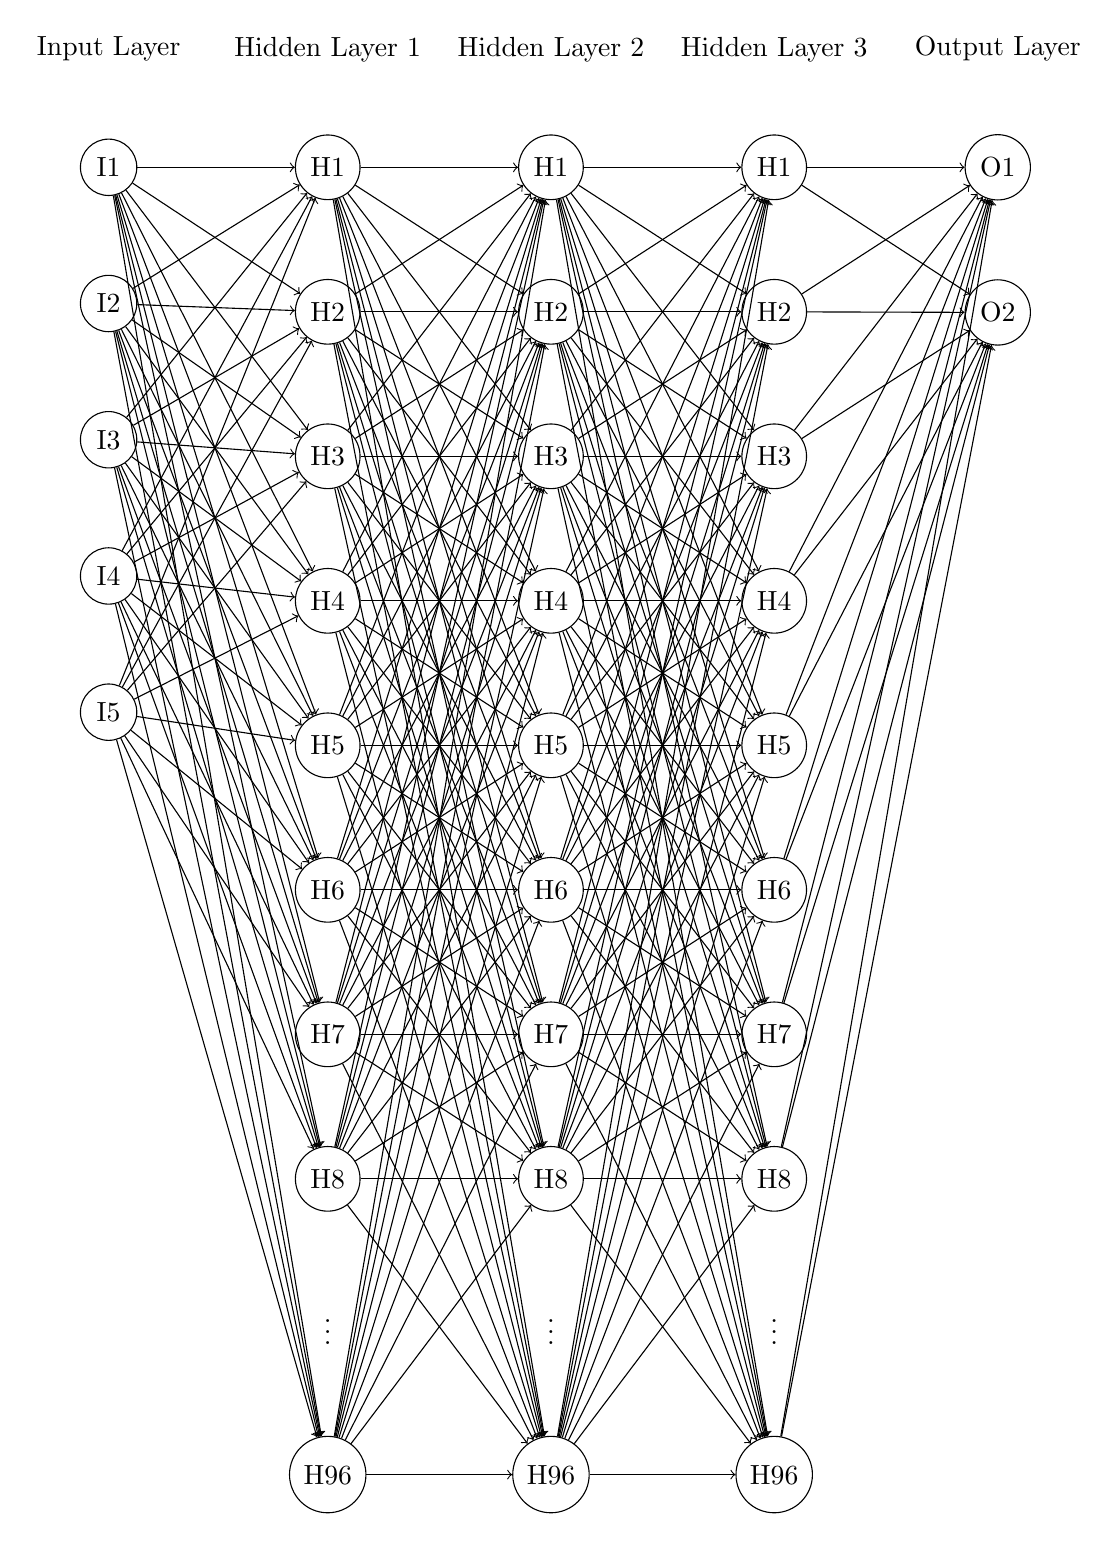
\begin{tikzpicture}[
        node distance=1cm,
        every node/.style={circle, draw, minimum size=0.6cm},
        layer/.style={rectangle, draw=none, fill=none, minimum size=0.5cm}
    ]
    
    % Input Layer
    \node (I1) {I1};
    \node (I2) [below=of I1] {I2};
    \node (I3) [below=of I2] {I3};
    \node (I4) [below=of I3] {I4};
    \node (I5) [below=of I4] {I5};
    
    % Hidden Layer 1
    \node (H1) [right=of I1, xshift=1cm] {H1};
    \node (H2) [below=of H1] {H2};
    \node (H3) [below=of H2] {H3};
    \node (H4) [below=of H3] {H4};
    \node (H5) [below=of H4] {H5};
    \node (H6) [below=of H5] {H6};
    \node (H7) [below=of H6] {H7};
    \node (H8) [below=of H7] {H8};
    \node (H9) [below=of H8, draw=none] {\vdots};
    \node (H10) [below=of H9] {H96};
    
    % Hidden Layer 2
    \node (H11) [right=of H1, xshift=1cm] {H1};
    \node (H12) [below=of H11] {H2};
    \node (H13) [below=of H12] {H3};
    \node (H14) [below=of H13] {H4};
    \node (H15) [below=of H14] {H5};
    \node (H16) [below=of H15] {H6};
    \node (H17) [below=of H16] {H7};
    \node (H18) [below=of H17] {H8};
    \node (H19) [below=of H18, draw=none] {\vdots};
    \node (H20) [below=of H19] {H96};
    
    % Hidden Layer 3
    \node (H21) [right=of H11, xshift=1cm] {H1};
    \node (H22) [below=of H21] {H2};
    \node (H23) [below=of H22] {H3};
    \node (H24) [below=of H23] {H4};
    \node (H25) [below=of H24] {H5};
    \node (H26) [below=of H25] {H6};
    \node (H27) [below=of H26] {H7};
    \node (H28) [below=of H27] {H8};
    \node (H29) [below=of H28, draw=none] {\vdots};
    \node (H30) [below=of H29] {H96};
    
    % Output Layer
    \node (O1) [right=of H21, xshift=1cm] {O1};
    \node (O2) [below=of O1] {O2};
    
    % Connections
    \foreach \i in {1,2,3,4,5}
        \foreach \j in {1,2,3,4,5,6,7,8,10}
            \draw[->] (I\i) -- (H\j);
    
    \foreach \i in {1,2,3,4,5,6,7,8,10}
        \foreach \j in {11,12,13,14,15,16,17,18,20}
            \draw[->] (H\i) -- (H\j);
    
    \foreach \i in {11,12,13,14,15,16,17,18,20}
        \foreach \j in {21,22,23,24,25,26,27,28,30}
            \draw[->] (H\i) -- (H\j);
    
    \foreach \i in {21,22,23,24,25,26,27,28,30}
        \foreach \j in {1,2}
            \draw[->] (H\i) -- (O\j);
    
    % Layer labels
    \node[layer] at ($(I1)!0!(I5) + (0,1.5cm)$) {Input Layer};
    \node[layer] at ($(H1)!0!(H10) + (0,1.5cm)$) {Hidden Layer 1};
    \node[layer] at ($(H11)!0!(H20) + (0,1.5cm)$) {Hidden Layer 2};
    \node[layer] at ($(H21)!0!(H30) + (0,1.5cm)$) {Hidden Layer 3};
    \node[layer] at ($(O1)!0!(O2) + (0,1.5cm)$) {Output Layer};
    
    \end{tikzpicture}
\end{center}

\newpage
\begin{itemize}
    \item \textbf{Input Layer:}
    \begin{itemize}
        \item \textbf{Description:} This is the first layer of the neural network. It inputs the row data or features of the dataset into the model.
        \item \textbf{Structure:} This consists of n Neurons where n is the number of features / columns in the dataset.
        \item \textbf{Function:} Data entry without performing computations.
    \end{itemize}

    \item \textbf{First Hidden Layer:}
    \begin{itemize}
        \item \textbf{Activation Function:} Rectified Linear Unit (ReLU)
        \item \textbf{Definition:} \( f(x) = \max(0, x) \)
        \item \textbf{Purpose:} Introduces non-linearity, mitigates the vanishing gradient problem, and allows the model to learn complex patterns.
    \end{itemize}

    \item \textbf{Second and Third Hidden Layers:}
    \begin{itemize}
        \item \textbf{Activation Function:} Sigmoid
        \item \textbf{Definition:} \( f(x) = \frac{1}{1 + e^{-x}} \)
        \item \textbf{Purpose:} Maps input values to a range between 0 and 1, useful for learning intermediate representations and refining features.
    \end{itemize}

    \item \textbf{Final Hidden Layer:}
    \begin{itemize}
        \item \textbf{Activation Function:} Softmax
        \item \textbf{Definition:} \( f(x_i) = \frac{e^{x_i}}{\sum_{j} e^{x_j}} \) for each class \( i \)
        \item \textbf{Purpose:} Converts raw output scores into probabilities, providing a probability distribution over possible classes, crucial for predicting customer churn.
    \end{itemize}

    \item \textbf{Output Layer:}
    \begin{itemize}
        \item \textbf{Structure:} Consists of two neurons, each representing one class: churn and non-churn.
        \item \textbf{Function:} Uses probabilities from the Softmax function to determine the class with the highest likelihood.
        \item \textbf{Loss Function:} Cross-Entropy
        \begin{itemize}
            \item \textbf{Definition:} The cross-entropy loss for a single instance is defined as \( L = -\sum_{i} y_i \log(p_i) \), where \( y_i \) is the true label (1 for the correct class, 0 otherwise) and \( p_i \) is the predicted probability for class \( i \).
            \item \textbf{Purpose:} Measures the performance of the model by comparing predicted probabilities to actual class labels. It penalizes the model more when the predicted probability for the true class is low, encouraging the model to assign higher probabilities to the correct class.
            \item \textbf{Advantages:} Cross-entropy is particularly effective for classification tasks as it provides a smooth gradient, which is beneficial for optimization algorithms like gradient descent.
        \end{itemize}
    \end{itemize}
\end{itemize}

\subsection{Training}

\begin{itemize}
    \item \textbf{Loss Function:} Cross-Entropy
    \begin{itemize}
        \item \textbf{Purpose:} Suitable for classification tasks, it measures model performance by comparing predicted probabilities to actual class labels, penalizing divergence from actual classes.
    \end{itemize}
\end{itemize}

\section{Activation Functions}

\section{Mathematical Formulation}

\section{Comparison of Activation Functions}

\section{References}
\bibliographystyle{plain}
\bibliography{references}

\end{document}